\documentclass[conference, 12pt]{IEEEtran}
%\documentclass[twocolumn, a4paper]{article}
\usepackage{verbatimbox}
\usepackage{url}
\usepackage{subcaption}
%%%%%%%%%% verbatim related
\usepackage{fancyvrb}
%\usepackage{fixltx2e}
\fvset{framesep=2mm,fontsize=\scriptsize,framerule=.1mm,numbersep=1mm,commandchars=\\\{\}}
\usepackage[usenames,dvipsnames]{color}

\newif\ifrev
%%%%%%%%%%%%%%%%%%
% COMMENT OUT NEXT LINE TO HIDE comments
\revtrue
%%%%%%%%%%%%%%%%%%

\newcommand{\urlwofont}[1]{\underline{\urlstyle{same}\url{#1}}}

\ifrev
  \newcommand{\yanyan}[1]{{\color{blue} [Yanyan: #1]}}
  \newcommand{\dave}[1]{{\color{red} [Dave: #1]}}
\else
  \newcommand{\yanyan}[1]{}
  \newcommand{\dave}[1]{}
\fi

\usepackage[utf8]{inputenc}
\usepackage{tcolorbox}
\pagestyle{plain}
\title{Confusion in Coding and \\Comprehension Models to Overcome it}

\author{\\
\\
David Stout \\

University of Colorado Colorado Springs \\

October 2018}
\date{}

%\usepackage{natbib}
\usepackage{graphicx}
\usepackage{fancyvrb} %needed to center verbatim text

% Keywords command
\providecommand{\keywords}[1]
{
  \small	
  \textbf{\textit{Keywords---}} #1
}
\newcommand{\comm}[2]{}
\begin{document}

\maketitle
\begin{abstract}
 \comm{\yanyan{These first few sentences wander kinda off topic. Need to get to the point in abstract.}} \ In
 the realm of Computer Science, where the logic in code can be wildly 
different from one developer to the next, the potential for confusing patterns is abundant. As source code has exploded in individual projects from a few dozen lines to 
hundreds of thousands of lines, and the need for teams of developers has become more commonplace, that possibility of increased
confusion has continued to rise exponentially. This increased potential for confusion has created a higher overhead on  
debugging, re-factoring, and maintenance of projects. Reducing that 
potential for confusion and understanding the underlying cause of confusion is what the field of Source Code Comprehension is all about.
This paper explores the current comprehensional models accepted by the community, and looks at the methods for increasing code interpretation by measuring cognitive understanding in
those program comprehension models, exploring the creation of software clarity metrics, and following coding standards through style guides. In the interest of the completion of source comprehension understanding, we also look at the inversely related field of code obfuscation and how it can be reversed for better code comprehension. By understanding most of the methods that are currently available in code comprehension, it becomes apparent that there is still room for newer methods of identification and solutions to make source code less confusing.
\comm{\yanyan{You could mention something like "there is still room for newer methods of identification and solutions to make source code less confusing".}}\
\end{abstract}
\keywords{Code comprehension, software readability, clarity metrics, style guides, obfuscation}
\section{Introduction}
\begin{quote}
%"If confusion leads to knowledge, then I must be a genius."\begin{flushright}- Larry Leissner\end{flushright}
%     "We often confuse what we wish for with what is." \begin{flushright}- Neil Gaiman \end{flushright}
\end{quote}

Confusion is something that everyone faces in life at some point. 
Whether it is rooted in unclear instructions, 
convoluted rules, or the actions of others, confusion is an 
obstacle that must be overcome to achieve the goals 
we want. How we choose to perceive the world around us has a significant impact in our daily
lives, and unless the choices are very clear (stop or go, on or off, etc.) the potential for confusion 
is always present. This can be a significant problem when we confuse the intent of source code while
developing software. 

Computer science is no stranger to confusing code, and 
sometimes even the intent is to make code inherently 
confusing for security and privacy. Code confusion is when people, whether 
by design or by happenstance, misunderstand the functionality or intent of source 
code. Even misunderstandings of small pieces of the source 
code can lead to larger misunderstandings of the program code as a 
whole. 

Code comprehension is the process by which a developer creates a 
mental model of a software system’s architecture, 
behaviors, and actions based upon the source code. With the increase of more developers on projects, the need
for a uniform understanding of the source between developers is key to the successful development of
software.
As code comprehension is such a vital area for moving forward in 
a software development life-cycle, then it stands to reason that 
making comprehension a more natural process by improving upon the source code is a worthwhile endeavor.

Zokaites describes software as "a 
natural language that must be understood by two separate entities 
for two different purposes"~\cite{zokaites_writing_2002}. One entity is the 
compiler or interpreter that transfers source code into machine 
language, and the other being is developers who need to 
maintain, utilize and create the application. The main difference between programming languages
and natural languages is that
in natural languages 
there is ambiguity that people must interpret. However, programming languages communicate a task to be conducted by a
computer, and thus need to be precise and without any ambiguity.

This does not have an effect on compilers and
interpreters handling confusing code, however problems occur when 
developers are attempting to debug, re-factor, and maintain source 
code. As in the case of \textit{reversed subscript} described by 
Gopstein et al~\cite{gopstein_prevalence_2018}, as shown in Figure~\ref{fig:reversed},
each method individually is seen as producing the same result
from the compiler's view, but the developer often become confused by 
the reversed subscript code snippet on the left. The 
developer can believe that there is a different interpretation when 
the subscript is reversed, rather than when it is not.
These unintentional misinterpretations are what lead 
to code confusion.

\begin{verbbox}[\scriptsize]
void main() {            void main() {
char V1 = 2["qwert"];    char V1 = "qwert"[2];
printf("\%c\n", V1);     printf("\%c\n", V1);
}                        }
\end{verbbox}

\begin{figure}[ht]
\begin{tcolorbox}
\centering
\theverbbox\qquad
\end{tcolorbox}
\caption{Reversed Subscript (left) VS Normal Subscript (right) }
\label{fig:reversed}
\end{figure}



 

%\subsection{Impact of Code Comprehension}\label{sec-impact}
Because software projects and languages are being developed as larger and more complex systems, source code confusion is becoming more
prevalent in a wide array of applications in production. In 
\textit{Code Complete} \cite{mcconnell_code_2004}, McConnell states that industry
averages between 15-50 errors per 1000 lines of delivered code. Therefore, as the number of lines
of code in projects grows so does the amount of errors. By understanding the code thoroughly developers can reduce the potential for errors due to code confusion, which increases the need for better code comprehension methods.

Just during maintenance and re-factoring stages developers spend a major 
portion of their time, approximately 60-90\%~\cite{ward_program_nodate}, on simply trying to understand the
source code. In fact many development teams would
benefit greatly, reducing a significant portion of the 
maintenance and re-factoring overhead by simply making their 
software easier to comprehend.

There are more developers on projects than ever before, and the impact of 
misinterpreting the outcome of code portions can create cascading effects that ripple throughout the project.  With
each module of a program depending on the results of others, a single error can create a ripple effect throughout the entire program.
At implementation time, this can cause a massive overhead in debugging code because the compiler would not 
throw any errors, but the results will be affected all down the line.

Software maintenance is a very costly, broad, and complicated process 
as it requires very deep understanding of the target system source 
code. Moreover, professional
developers must be familiar with the system undergoing change in order to accomplish
the required maintenance tasks \cite{alhindawi_degree_nodate}.

For example, a developer at the financial code supplier IMMUNIO, used a fork to create additional
processes. This developer interpreted an if/then condition incorrectly which was supposed to test for when
the program could stop forking. Since the program continued to fork endlessly, the whole system was taken
down due to the hundreds of connections to the back-end eating up resources. Since the communications were
so bogged down, this meant that their clients were not able to complete transactions quickly enough and
lost millions of dollars \cite{sherman_21_nodate}. 

Also, a similar situation happened in 2012 when the Knight Capital Group needed to replace code that was
years-old but no longer used. Due to a misunderstanding, the flag that was used to call the old code was 
repurposed and sent to the servers without copying over the new code. This "glitch" ended up being
propagated to all the servers when technicians took the code off of the other servers. In 45 minutes the
company sold all the stock it had bought that morning ending in a net loss of 440 million dollars
\cite{sherman_21_nodate}.

With the inter-connectivity of modules in large projects, code comprehension is a major time and cost investment for 
developers. The ability to understand
pre-existing source code is one of the most important elements 
of a continuously successful software
project~\cite{gopstein_understanding_2017}. Take the Linux kernel 
development for example, with hundreds of thousands of lines of 
code and dozens of inter-working modules (as shown in 
 Figure~\ref{fig:kern}), a single confusing bit of 
code can create errors that ripple throughout the entirety of 
the system and would be incredibly hard to track down. 

\begin{figure*}%[htbp]
\centering
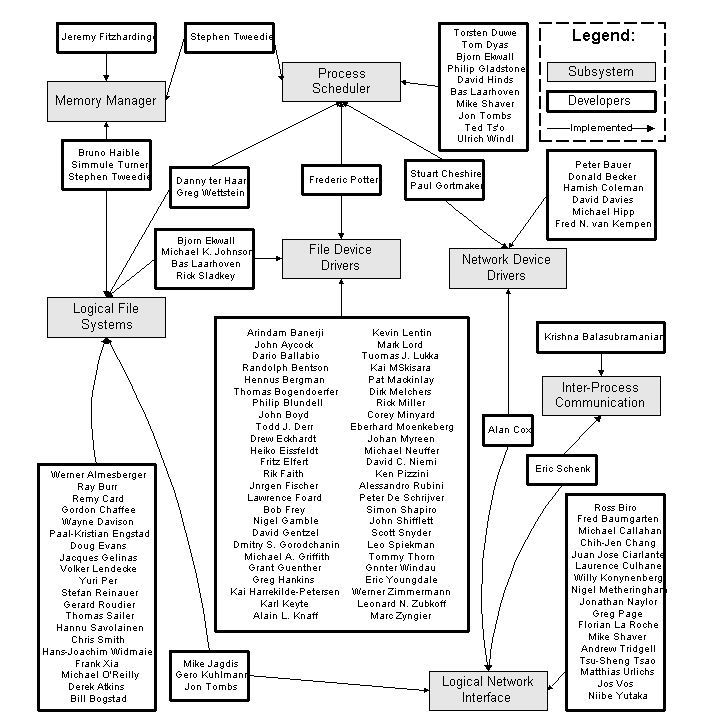
\includegraphics[scale=.75]{images/LinuxKernel}
\caption{Modules of the Linux Kernel and assigned developers \cite{noauthor_conceptual_nodate}}
\label{fig:kern}
\end{figure*}

Code confusion creates an expensive overhead cost to developers 
and is an acknowledged problem in the community 
that has had a number of suggested solutions proposed, but has 
never had a panacea solution. Simply
being able to reliably identify and remove code that can cause 
misunderstandings will enhance productivity and reduce maintenance 
costs~\cite{gopstein_understanding_2017}.

%\subsection{Objective}
This paper will explore the effectiveness of the methods for 
improving code comprehension suggested by the 
measurement of cognitive comprehension in program comprehension 
models, the creation of software clarity metrics to 
increase software readability, the use of coding style guides in 
multi-developer projects, and the inverse relation of
code obfuscation in security. Analysis of the methods that are 
currently available will show that there is still room 
for newer methods of identifying confusing code and the 
combination of current solutions that can greatly increase source 
code comprehension.

%\subsection{Organization}
The following organization method is used to present this research. Section I  
details what code 
comprehension is and why it continues to
be an important field of research. Section~\ref{sec-models} then 
discusses the main three models of code
comprehension, examining their 
common features and differences.  In Section~\ref{sec-current}, 
we will present the
current research methods and tools used to increase code 
comprehension and examine the inversely related field of code obfuscation, and in Section~\ref{sec-compare} we will compare
these methods to determine 
how we can use these principles to affect change towards code 
comprehension. Finally, in Section~\ref{sec-conclude} we will give 
a summary from all the research into code comprehension and where we can go
in future work.

\begin{figure*}[ht!]
\centering
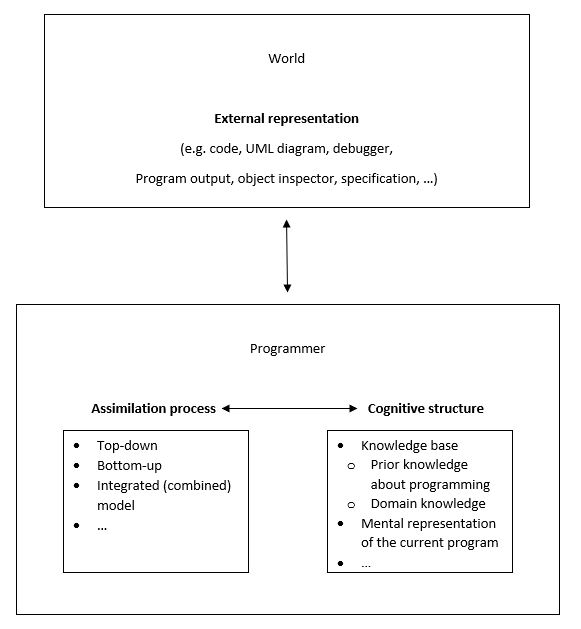
\includegraphics[scale=0.85]{images/ProgramCompModels}
\caption{Commonalities in comprehension models. \cite{noauthor_pdf_nodate}} 
\label{fig:models}
\end{figure*}

%\section{Literature Review}\label{sec-comprehend}
%\yanyan{I feel this section still belongs to intro. You could cut
%these sentences and place them in appropriate places in intro
%where you need more supporting evidence.}
Code comprehension is the process by which a developer creates a 
mental model of a software system’s architecture, 
behaviors, and actions based upon the source code. With the increase of more developers on projects, the need
for a uniform understanding of the source between developers is key to the successful development of
software.
As code comprehension is such a vital area for moving forward in 
a software development life-cycle, then it stands to reason that 
making comprehension a more natural process by improving upon the source code is a worthwhile endeavor.

Just during maintenance and re-factoring stages developers spend a major 
portion of their time, approximately 60-90\%~\cite{ward_program_nodate}, on simply trying to understand the
source code. In fact many development teams would
benefit greatly, reducing a significant portion of the 
maintenance and re-factoring overhead by simply making their 
software easier to comprehend. 

\begin{figure*}%[ht]
\centering
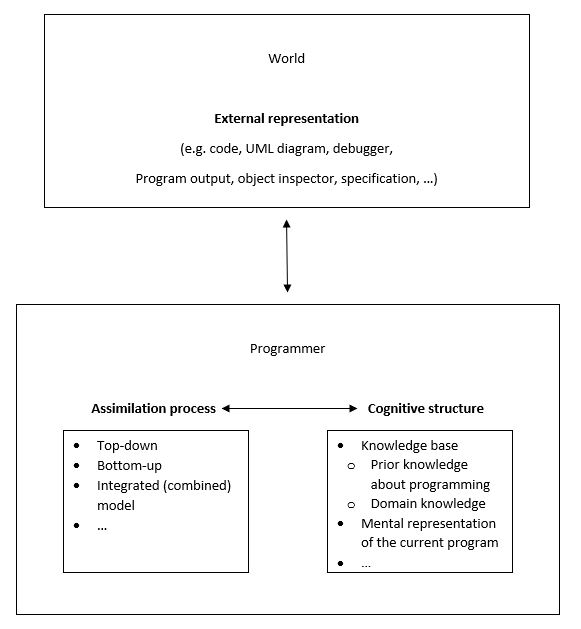
\includegraphics[scale=0.85]{images/ProgramCompModels}
\caption{Commonalities in comprehension models.} 
\label{fig:models}
\end{figure*}

Software maintenance is a very costly, broad, and complicated process 
as it requires very deep understanding of the target system source 
code. Moreover, professional
developers must be familiar with the system undergoing change in order to accomplish
the required maintenance tasks \cite{alhindawi_degree_nodate}. 
\yanyan{This paragraph lacks some logic. What's the purpose? Should
some of these sentences be spread out in other paragraphs as 
examples or supporting evidence?}


\section{Literature Review}\label{sec-models}
There are varying models of code comprehension that have been
suggested over the years. Most contain some 
common elements, as shown in Figure \ref{fig:models}~\cite{noauthor_pdf_nodate}. 



In this paper we will focus on the three most important:
\begin{itemize}
    \item The Top-down model
    \item The Bottom-up model
    \item The Integrated (combined) model
\end{itemize}

The \textbf{Top-down model} describes a process that consists of applying knowledge about the domain of the
program and then applying this knowledge to the structure of the 
code~\cite{noauthor_pdf_nodate}. This
process of assimilating data is driven by recognizing beacons, or sets of features that typically
indicate the occurrence of certain structures or operations within the code, as described by Brooks~\cite{brooks_towards_1983}. 
Top-down comprehension is a functional understanding of the code, starting
with the big picture and then breaking down the source code from there into smaller segments in order
to understand the whole.

The \textbf{Bottom-up model} describes an assimilation process in 
which programmers start with individual code
statements, and chunk or group these into higher level abstractions. 
The process is then repeated at
successively higher levels until a complete mental representation of the program is formed~\cite{noauthor_pdf_nodate}. 
There have been investigations into the human factors of code
comprehension, showing that minimally small patterns in code can 
and do confuse programmers~\cite{gopstein_understanding_2017, 
gopstein_prevalence_2018}. Generally
seen as a method of chunking microstructures in the code into macrostructures to comprehend the
program flow, Bottom-up modelling uses environmental information to form a perception of the whole by
identifying individual base elements in great detail in order to link them to greater and greater
subsystems. 

Some authors do not accept that there is a dominance of either top-down or bottom-up
comprehension, choosing instead to believe that the developer switches between the two models as the
situation needs. This ideology is made clear in the 
\textbf{Integrated model}, which is a combined model of both the Top-down and Bottom-up approaches \cite{noauthor_pdf_nodate}. As the developer goes through the
assimilation process of comprehending the source code, they switch from a functional understanding of the
program, to a control-flow understanding as is needed for greater overall comprehension. This approach
seems to be a more intuitive process and depends on the developer's previous experience and the berth of
their knowledge base.

By understanding these comprehension models, researchers are able to evaluate the best methods for measuring code comprehension, create software clarity metrics for automated comprehension tools, and develop better coding style guides. We will use these models to help organize and classify the current research.

\section{Current Research}\label{sec-current}
The effort to enhance source code comprehension has been ongoing since the 
1980s \cite{brooks_towards_1983,letovsky_cognitive_1987} and continues to be an active research field today. In this section we will examine the newer methods of measuring comprehension using comprehension models, inspect current software clarity metrics and the tools in place that use them, review the use of coding style guides in development studios, and study the art of obfuscation and how it can be reversed to help increase code comprehension.

\subsection{Measurement of Comprehension}
Most modern software programs are so complex, relying on multiple modules and libraries, that they become very difficult to understand in their entirety by a programmer. Instead, programmers must rely on a set of cognitive processes that aid in seeking, filtering, and
shaping relevant information for a given programming task \cite{siegmund_measuring_2017}. These comprehension models are described in Section~\ref{sec-models} as: top-down, bottom-up, and integrated.

Siegmund et al \cite{siegmund_understanding_2014}, uses a functional magnetic resonance imaging (fMRI)
scanner to show that bottom-up chunking techniques increase subjects overall code comprehension. The
researchers were able to replicate their original results, and further solidify their original findings of
the effectiveness of chunking techniques in bottom-up comprehension models \cite{siegmund_measuring_2017,
siegmund_understanding_2014}. As shown in Figure \ref{fig:fMRI}, their experiments found that the 
cognitive centers of the brain activated more intensely when using chunking methods of bottom-up
comprehension, than when using top-down comprehension models. Their results showed that the areas of the
brain linked to cognition and understanding (Brodmann areas), are more active during chunking practices
than they are during top-down comprehension. 

Yeh et al \cite{yeh_detecting_2017}, also found that when using an electroenchephalogram (EEG) subjects
had smaller alpha and theta band magnitudes during comprehension of non-confusing code snippets versus
confusing code snippets. The non-confusing micro-patterns were presented in a method that was similar to
bottom-up models, where the snippet was small enough that the participants of the experiment were able to
determine the smaller pieces (chunks) first and apply that knowledge to the idea that made up the overall
purpose of the program. Their experiment was setup to measure the difference in theta and alpha band
magnitudes over the 8 channels that are related to cognitive load, as indicated by the red circle shown in
Figure \ref{fig:EEG}. The results showed that smaller non-confusing code patterns were easier for subjects
to understand and these findings fit well with the bottom-up approach of comprehension models.

While the current research in Software comprehension seems to lead towards a bottom-up model of
comprehension being the most effective \cite{siegmund_measuring_2017, siegmund_understanding_2014, yeh_detecting_2017, nakagawa_quantifying_2014}, it should be noted that source code is a language and can
be read as such. Angosto et al \cite{angosto_pdf_nodate} studied general reading comprehension when the
subject does not have prior knowledge of the material. In their experiments it was shown that without
prior knowledge that a broad overview (top-down model approach) of the material was best suited to the
subject's cognitive understanding. 

These experimental results show that a version of the bottom-up comprehension model seems to work best when reading source with a bit of prior knowledge of the code, and if there is no prior knowledge of the source a top-down model works well. Combining the findings of this research would suggest that an integrated model of comprehension would be a future area of research in code comprehension. As research continues in this area, there will be a more solid confirmation of what types of comprehensional model will be the most useful in designing automatic tools and metrics to make the job of software readability easier.

\begin{figure}[ht]
\centering
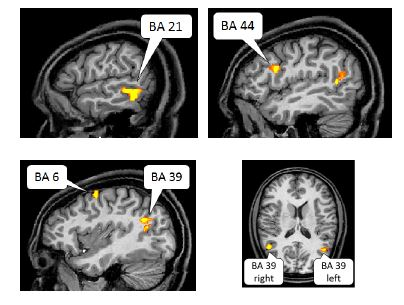
\includegraphics[scale=0.75]{images/fMRI}
\caption{Functional MRI scans that show activation in the Brodmann-areas during bottom-up comprehension.}
\label{fig:fMRI}
\end{figure}

\begin{figure}[ht]
\centering
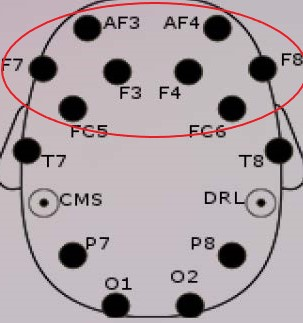
\includegraphics[scale=0.75]{images/EEG}
\caption{Electrode positioning of EEG headset in Yeh et al experiment with the 8 cognitive load channels highlighted.\cite{yeh_detecting_2017}}
\label{fig:EEG}
\end{figure}



\subsection{Software Clarity Metrics}
To improve program comprehension, there has also been research done in software readability and clarity
metrics. Metrics are a measurement by which an attribute's state is determined. Using these determinations
we can gauge the effectiveness of software readability and comprehension applications, with the hopes of
improving the behavior that is desired. Maurya states that the factors that influence understandability
characteristics in comprehending software are an internal software quality and an internal process of
human influences\cite{maurya_software_nodate}. As shown in Figure \ref{fig:models}, the programmers
knowledge base and mental representation of the program under analysis help to aid the assimilation
process during comprehension.  
  
Comprehension of source code can often be equated to the effective readability of the source, meaning that
the easier it is for developers to read the code tends to directly effect how easily the developers
understand it \cite{dorn_general_nodate}. Work on software clarity metrics has shown that factors such as
the number of identifiers, the number of
statements, and the amount of branching have an impact on code comprehension~\cite{brooks_towards_1983}.

In more current research the length of identifiers was not shown to have an impact on comprehension, while
the amount of characters per line was shown to have a significant impact \cite{buse_metric_2008}. By improving the metrics that are used to determine the effectiveness of comprehension in specific attributes
commonly used in source code, we are able to write more efficient automated methods for determining a
programs overall readability.  
\subsection{Coding Style Guides}
A rather simple method of ensuring better program comprehension in a project is to follow a programming
language style guide. Each coding style is different because it is how a programmer's code is assembled to
look and is often influenced by the developer’s particular experiences (IDEs used, etc.) and can even vary
from language to language. Coding style guides provide an overarching standard methodology for the layout
and the usage for various pieces of language functionality in a project. An example from the Google C++ style guide is shown in Figure \ref{fig:style}.

\begin{figure}[ht]

\begin{tcolorbox}

\scriptsize 
\begin{Verbatim}
     \textbf{\textcolor{OliveGreen}{(a) Bad initialization:}}                             
1. int i;          
2. i = f();
3. //bad - initialization separate
   //      from declaration
     \textbf{\textcolor{OliveGreen}{(b) Good initialization:}}
1. int j = g();
2. //Good - initialization includes declaration
\end{Verbatim}
\end{tcolorbox}

\caption{Excerpt from Google C++ coding style guide regarding the declaration and initialization of local variables \cite{google_google_2011}.}
\label{fig:style}
\end{figure}


\begin{figure*}[!ht]
\begin{tcolorbox}

\scriptsize 
\begin{Verbatim}
   
   private void CalculatePayroll(SpecialList, employeeGroup) \{
     while(employeeGroup.HasMore())\{
         employee = employeeGroup.GetNext(true);
         employee.UpdateSalary();
         DistributeCheck(employee);
     \}
   \}    
\end{Verbatim}
\end{tcolorbox}
\caption{An example of source code containing vulnerability.
\label{fig-blind}}
\end{figure*}

Style guides help to ensure that all programmers adhere to the same coding standard, by keeping all the pieces 
of the project consistent. This consistency allows for a quicker understanding of the source code by
all members of the project. Using standards and heavily documenting the program helps to ensure future developers are well equipped to understand the source.

Coding style guides are popular in industry and large scale open-source projects 
\cite{google_google_2011,weinberger_google_2011,doland_c_1994,torvalds_linux_nodate, van_rossum_pythonstyle-pep_2001} because they provide a map that 
allows anyone to quickly get into the meaning of the code by providing detailed directions to follow. They are more 
than just a document, and have helped to change the way that software projects are developed by providing
a uniform practice which allows any developer to just jump right in on the project
\cite{gale_collaborative_1996}.

A good code style guide is like following a turn-by-turn GPS to a destination since
there is no need to take the road less traveled, instead it is guaranteed that instead the most direct route to the final goal is taken. Style guides help new 
developers to the team catch up quickly \cite{google_google_2011}, provide significantly less overhead maintenance \cite{torvalds_linux_nodate}, and help to keep all 
modules looking cohesive \cite{doland_c_1994}. With the knowledge of what practices work best, newer style guides may be created to maximize the potential for source code comprehension.


\subsection{Obfuscation}
After researching all efforts that have gone into making code easier to understand it is worth noting that not all developers wish to make their code easier to read. In fact, many strive to make their code as
difficult as possible to prevent reverse engineering and theft of their coding ideas. In the fast
paced world of software development, many companies rely on confusion in their code in order to increase security from hacking and code theft. 

Source code obfuscation is essentially a protection mechanism, for vulnerable code as shown in Figure \ref{fig-blind}, that is widely used to limit the possibility of malicious reverse
engineering or attack activities on a software system \cite{ceccato_effectiveness_2009}.
Obfuscation is a method that is inversely related to code comprehension, so much that the ideals of
obfuscation in themselves can help us to understand what makes code confusing in the first place.  
Obfuscated code is by design confusing code, and the methods that are used to ensure it is confusing
can lead to a better understanding of unintentionally confusing code.

As shown in Figure \ref{fig:Transforms}, obfuscation transformations can be classified into three groups: \textbf{layout obfuscations} which remove
relevant information from the code without changing its behavior; \textbf{data obfuscations} which transform application
data and data structures (e.g., data encoding, data splitting); and, \textbf{control-flow obfuscations} which alter the original flow of the application \cite{collberg_taxonomy_1997}.

The technique of obfuscation that is of particular interest is identifier renaming, which is an instance of layout obfuscation.
It removes relevant information from the code by changing the names of classes, fields and operations into
meaningless identifiers \cite{ceccato_effectiveness_2009}, as shown in Figure \ref{fig:test}. By reversing this process, it is apparent that identifier naming conventions can increase software clarity and overall code comprehension.

\begin{figure*}[ht]
\centering
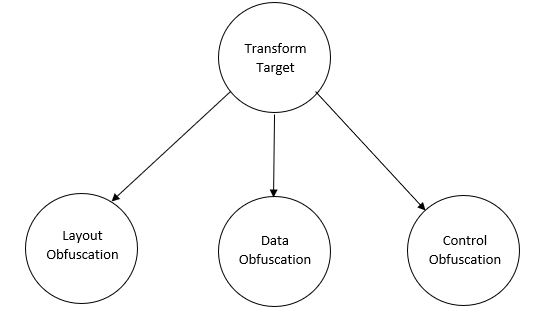
\includegraphics[scale=.7]{images/Obfuscate}
\caption{Classifications of Obfuscation Transforms}
\label{fig:Transforms}
\end{figure*}

\begin{figure*}
\begin{tcolorbox}
\centering
\begin{subfigure}{.5\textwidth}
  \centering
  %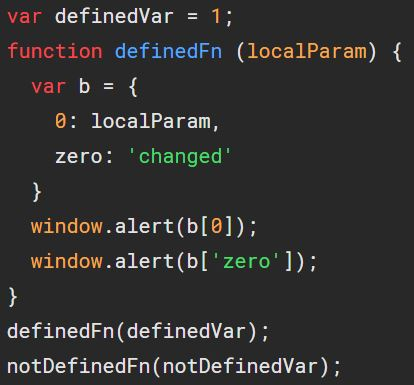
\includegraphics[width=.6\linewidth]{images/ID1}
  \begin{Verbatim}
  var definedVar = 1;
  function definedFn(localParam) \{
    var b = \{
      0: localParam,
      zero: 'changed'
    \}
    window.alert(b[0]);
    window.alert(b['zero']);
  \}
  definedFn(definedVar);
  notDefinedFn(notDefinedVar);
  \end{Verbatim}
  \caption{Normal Identifiers}
  \label{fig:sub1}
\end{subfigure}%
\begin{subfigure}{.5\textwidth}
  \centering
  %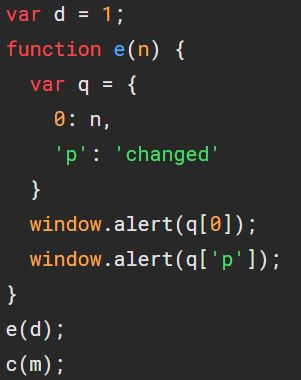
\includegraphics[width=.5\linewidth]{images/ID2}
  \begin{Verbatim}
  var d = 1;
  function e(n) \{
    var q = \{
      0: n,
      'p': 'changed'
    \}
    window.alert(q[0]);
    window.alert(q['p']);
  \}
  e(d);
  c(m);
  \end{Verbatim}
  \caption{Obfuscated Identifiers}
  \label{fig:sub2}
\end{subfigure}
\end{tcolorbox}
\caption{An example of Identifier Obfuscation}
\label{fig:test}
\end{figure*}
There is so much interest in the obfuscation of code that there are a number of contests in which the
sole purpose is to make the source code as confusing as possible. These contests span a majority of
languages and show that obfuscation is something that is not only possible, but desired in many facets
of the software development industry. The oldest contest that is still running is the International
Obfuscated C Code Contest (IOCCC)\footnote{\url{https://www.ioccc.org/}}, which has been around since 1984. The winners of the IOCCC strive to
create code that is functional but incredibly hard to follow, as seen in Figure \ref{fig:IOCCC}. Winners of
the contest often use little known tricks, such as using the C preprocessor to do unintended things, or
they tend to avoid using common constructs that are available in C in favor of more obscure methods 
that achieve the same results.  


\begin{figure}[!ht]
\scriptsize
\centering
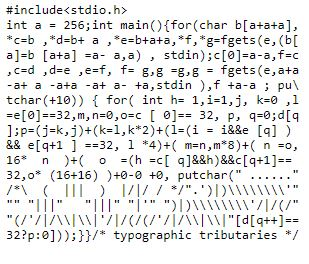
\includegraphics[scale=1.0]{images/IOCCC}
\begin{comment}
\begin{Verbatim}[frame=none]
#include<stdio.h>
int a = 256;int main()\{for(char b[a+a+a],
*c=b ,*d=b+ a ,*e=b+a+a,*f,*g=fgets(e,(b[
a]=b [a+a] =a- a,a) , stdin);c[0]=a-a,f=c
,c=d ,d=e ,e=f, f= g,g =0,g = fgets(e,a+a
-a+ a -a+a -a+ a- +a,stdin ),f +a-a ; pu\\
tchar(+10)) \{ for( int h= 1,i=1,j, k=0 ,l
=e[0]==32,m,n=0,o=c [ 0]== 32, p, q=0;d[q
];j=k,k=l,m=n,n=o,p=(j)+(k* 2 )+(l =(i = 
e[ q]&&i ) &&e[q +1 ]== 32,l*4)+(m* 8 )+(
16*  n  )+(  o  =(h =c[ q]&&h)&&c[q+1]== 
32,o* (16+16) )+0-0 +0, putchar(" ......"
/*\  (  |||  )  |/|/ / */".')|)\\\\\\\\'"
"" "|||"   "|||" "|'" ")|)\\\\\\\\'/|/(/"
"(/'/|/\\|\\|'/|/(/(/'/|/\\|\\|"[d[q++]==
32?p:0]));\}\}/* typographic tributaries */
\end{Verbatim}
\end{comment}
\caption{A winner of the 2018 IOCCC \cite{noauthor_international_nodate}.}
\begin{comment}
\yanyan{ 
Also please check some of the backslashes. 
They need to have an escape char.}\end{comment}

\label{fig:IOCCC}
\end{figure}

In quantifying program obfuscation, we can also quantitatively approach code defactoring which leads us
towards increased code comprehension\cite{anckaert_program_2007, capiluppi_code_2012}. By reversing the
principles of obfuscating code we see that there are certain aspects that help to make
code really confusing and may be able to update style guids to help remove those practices in production
code when we wish to increase code comprehension. 
\section{Synthesis of Research}\label{sec-compare}
By examining the current research, we see that there is still a need for methods to increase code comprehension. By using current methods of neuroscience \cite{siegmund_measuring_2017, siegmund_understanding_2014, yeh_detecting_2017, nakagawa_quantifying_2014} it is possible to begin efforts to quantify the effectiveness of program comprehension models. As we begin to understand what comprehension model is best suited to understanding source code, we can design better metrics to measure the state of understanding specific attributes of code. Then when newer technologies are created, this process can continue to be refined and will help us to understand the best methodology to use for modeling code comprehension\cite{siegmund_measuring_2017}.

The attributes that lead to a higher rate of code comprehension can then be used to write newer and more robust coding style guides, as well as create automated applications that can evaluate source code ease of comprehension and identify confusing code sections for the refactor and maintenance periods. This will significantly reduce the overhead for developers who currently spend a large segment of their time trying to understand the code. The information can also be useful to researchers that wish to create more robust obfuscation tools, by identifying some key areas that need to be obfuscated.



\section{Conclusion}\label{sec-conclude}
Code comprehension is especially important in today’s environment of code reuse. Where instead of reinventing the wheel, developers are reusing code at a faster pace than ever before. While source code style guides, 
thorough commenting, and coding standards help make this an easier prospect there is no guarantee that they will be used on every project. The only guarantee is how the compiler will interpret the source, while the
human aspect is up to individual interpretation.

 Without being the original developer of the source,
future developers are relying on their comprehension of the source code. With our propensity for confusion, it is clear that there is a need for tools that can help with code comprehension. By using a combination of clarity metrics, code style guides, and deobfuscation methods code can become clearer and concisely interpreted by most developers. 


%\clearpage

%\nocite{*}
\bibliographystyle{ieeetr}
\bibliography{References2}
\end{document}
